
\documentclass[9pt,twoside]{pnas-new}

\articletype{RESEARCH ARTICLE}

\templatetype{pnasmathematics}

\graphicspath{{../output/}{./}}

\begin{document}

\title{Offshore in the Gray Zone: Georgian Elites, Post-Soviet Capital, and the Dual-Track Secrecy Strategy}

\author[a]{Naniko Kakonashvili}

\affil[a]{Program in Quantitative Social Science, Dartmouth College, Hanover, NH 03755}

\leadauthor{Kakonashvili}

\significancestatement{Cross-national studies of offshore finance typically treat each country as an independent observation. Using the ICIJ Offshore Leaks Database---five financial leaks covering over 810,000 entities---this study instead positions one small, geopolitically ambiguous post-Soviet state, Georgia, within a measured strategy space defined by Russian and Western European reference economies. Georgian-linked actors combine maximally opaque jurisdictions (British Virgin Islands, 46\% of entities) at rates approaching Russia's, while simultaneously using EU-adjacent Malta (26\%) at rates that exceed Russia's and approach Western European levels. Cosine-similarity analysis places Georgia closer to Russia (0.66) than to the EU average (0.45), yet its elevated intermediary concentration and EU-adjacent share distinguish it from both, indicating a hybrid strategy not captured by the binary post-Soviet/EU contrast.}

\authorcontributions{N.K. designed the study, performed all analysis, and wrote the paper.}
\authordeclaration{The author declares no competing interests.}
\correspondingauthor{Naniko Kakonashvili. E-mail: naniko.kakonashvili@dartmouth.edu}

\keywords{offshore finance $|$ tax havens $|$ oligarchy $|$ post-Soviet $|$ Georgia $|$ ICIJ}

\begin{abstract}
Do post-Soviet elites from small, geopolitically ambiguous states manage offshore wealth like Russian oligarchs or like their Western European counterparts? This paper investigates Georgian-linked actors in the ICIJ Offshore Leaks Database, comparing their offshore jurisdiction preferences, intermediary structure, and temporal incorporation patterns against Russian and EU reference groups. The database aggregates five leaks (Offshore Leaks 2013, Panama Papers 2016, Bahamas Leaks 2016, Paradise Papers 2017, Pandora Papers 2021) with entity records spanning roughly 1977--2020; the Georgian temporal analysis covers 1991--2018. Using five quantitative features (blacklisted-jurisdiction share, Shannon entropy of jurisdiction diversity, Herfindahl--Hirschman index of intermediary concentration, EU-adjacent jurisdiction share, and temporal recency), I construct offshore strategy vectors for Georgia, Russia, Latvia, Belarus, Germany, and France. Cosine-similarity analysis shows Georgia is closer to Russia (0.66) than to the EU average (0.45), with the strongest structural resemblance to Belarus (0.93). Yet Georgia's high EU-adjacent share (28.7\%) and elevated intermediary concentration ($\text{HHI}=0.068$, the highest in the comparison set) distinguish it from both Russia and Western Europe, evidencing a dual-track strategy. Georgian entity incorporations peak in 2014, two years after the Georgian Dream party's 2012 electoral victory, with a post-2016 decline coinciding with the Panama Papers release. The analysis is descriptive and comparative; it situates Georgia within the offshore strategy space rather than testing causal claims.
\end{abstract}

\dates{This manuscript was compiled on \today}
\doi{\url{www.pnas.org/cgi/doi/10.1073/pnas.XXXXXXXXXX}}

\maketitle
\thispagestyle{firststyle}
\ifthenelse{\boolean{shortarticle}}{\ifthenelse{\boolean{singlecolumn}}{\abscontentformatted}{\abscontent}}{}

\Firstpage

Offshore financial secrecy has been studied extensively for large economies. Roughly 8\% of global household financial wealth is held offshore, the bulk of it undeclared \cite{zucman2015}. Alstad{\ae}ter, Johannesen, and Zucman (2019), matching leaked offshore customer lists to Scandinavian administrative wealth records, establish that offshore tax evasion is steeply concentrated at the top of the wealth distribution---the richest 0.01\% of households evade roughly a quarter of their taxes, against under 5\% in random audits \cite{alstadsaeter2019}. This concentration is precisely why the offshore behavior of elites, rather than ordinary taxpayers, is the relevant object of study. Chang, Harrington, Fu, and Rockmore (2023) analyze the wealth-manager intermediary networks of ultra-high-net-worth individuals from Russia, China, the United States, and Hong Kong, finding scale-free network structures whose topologies diverge between democratic and autocratic regimes; Russian clients in particular concentrate their offshore business in a small number of boutique wealth-management firms, making those intermediaries a structural vulnerability \cite{chang2023}.

A broader cross-national perspective has emerged more recently. Chang, Harrington, and Rockmore (2025) examine offshore secrecy strategies across 65 countries, combining the ICIJ database with the World Justice Project Rule of Law Index, and show that elite strategies are contingent on home-country political conditions: elites from more corrupt countries diversify across multiple offshore centers, those facing high confiscation risk favor identity-concealing instruments, and those facing both pressures make heavier use of blacklisted havens \cite{chang2025}. That work treats countries largely as independent observations situated against governance indices. The present paper takes a complementary approach: rather than estimating population-level relationships, it positions a single focal state within a measured strategy space and quantifies its similarity to specific reference economies.

Georgia is an especially instructive focal case. It produced its oligarchic class through the same chaotic 1990s privatization economy as Russia, a process that converted Soviet-era state assets into highly concentrated private wealth across the post-Soviet space \cite{novokmet2018}, yet has since pursued the most active EU integration in the South Caucasus. Its emblematic actor, Bidzina Ivanishvili---founder of the ruling Georgian Dream party, former French citizen, and a fortune built in Russia---appears in both the Panama Papers and the Pandora Papers, embodying a wealth-holder suspended between two models. This positioning lets us ask whether a small post-Soviet state's offshore behavior tracks the Russian pattern, the EU pattern, or neither cleanly. To our knowledge no prior study has measured a single small post-Soviet state's offshore strategy as a vector and computed its similarity to both post-Soviet and EU reference economies; this is the gap the paper addresses.\Endparasplit

\section*{Data}

The primary dataset is the ICIJ Offshore Leaks Database, downloaded from \url{offshoreleaks.icij.org}, which consolidates five investigative leaks: Offshore Leaks (2013), Panama Papers (2016), Bahamas Leaks (2016), Paradise Papers (2017), and Pandora Papers (2021). The database covers 814,344 offshore entities and 771,315 officers across approximately 200 jurisdictions, with entity records spanning roughly 1977 through 2020. It is distributed as six CSV files representing nodes and relationships in a graph.

\textit{Unit of analysis.} In the original source, the unit is a graph element---a node (officer, entity, intermediary, or address) or a relationship edge. The unit of analysis in this study is the \textit{offshore entity linked to a nationality}: an entity is attributed to country $c$ if at least one officer coded to $c$ holds an \texttt{officer\_of} relationship to it. Four files are used: \texttt{nodes-officers.csv} ($n=771{,}315$), \texttt{nodes-entities.csv} ($n=814{,}344$), \texttt{nodes-intermediaries.csv} ($n=25{,}629$), and \texttt{relationships.csv} ($n=3{,}339{,}267$ edges).

\textit{Comparison design.} Six countries form two theoretical clusters. The \textit{post-Soviet focal group} is Georgia (the case of interest), Latvia (post-Soviet, EU member since 2004), and Belarus (post-Soviet, no EU integration). The \textit{anchor group} is Russia (post-Soviet anchor) and Germany and France (Western European baselines). Table~\ref{tab:sample} summarizes the analysis sample, including entity counts and the year range of incorporation dates used in the temporal analysis.

\begin{table}[h!]
\centering
\caption{Analysis sample. Entities are offshore shell companies linked to officers of each nationality via \texttt{officer\_of} edges.}
\label{tab:sample}
\begin{tabular}{lrrr}
Country & Entities & BL\% & EU-Adj\% \\
\midrule
Georgia  & 223    & 55.2 & 28.7 \\
Latvia   & 522    & 30.8 & 50.0 \\
Belarus  & 245    & 51.4 & 11.8 \\
Russia   & 11{,}328 & 60.0 & 13.4 \\
Germany  & 8{,}254  & 28.6 & 67.6 \\
France   & 4{,}749  & 33.7 & 58.0 \\
\bottomrule
\end{tabular}
\addtabletext{BL\% = share in blacklisted jurisdictions; EU-Adj\% = share in EU-adjacent jurisdictions. The Georgian subsample derives from 281 Georgian-coded officers. Full database spans $\sim$1977--2020; Georgian temporal analysis covers 1991--2018.}
\end{table}

\textit{Limitations and missingness.} Three limitations apply. First, \texttt{country\_codes} records how an officer was entered in leaked documents, not verified citizenship; Georgian name transliteration is also inconsistent across leaks, so attribution is approximate. Second, the database is a sample of convenience covering only what was leaked: absence of offshore records cannot be read as evidence of non-participation, and coverage is uneven across providers and across the post-2016 period. Third, missingness in the key temporal field is material: 36 of 223 Georgian-linked entities (16.1\%) have no parseable \texttt{incorporation\_date} and are excluded from the timeline ($n=187$ retained). With only 223 Georgian-linked entities, all findings are descriptive; no subgroup-level statistical inference is attempted.

\section*{Methods}

\textit{Jurisdiction classification.} Jurisdictions are grouped into three author-defined tiers, informed by FATF and EU listings of non-cooperative jurisdictions current as of 2023. \textit{Blacklisted} (high-secrecy) jurisdictions are British Virgin Islands, Panama, Seychelles, Bahamas, Samoa, Cook Islands, Belize, and Niue. \textit{EU-adjacent} (semi-transparent, tax-efficient but nominally regulated) jurisdictions are Malta, Bermuda, Isle of Man, Cayman Islands, and Mauritius. All others are classified as \textit{other}. Because blacklists are revised annually, this scheme is treated as a fixed analytical instrument rather than a claim about any single regulator's list.

\textit{Merge procedure.} The pipeline is implemented in pandas (notebook \texttt{01\_analysis\_and\_visualizations.ipynb}, helper \texttt{get\_country\_data}, lines $\sim$588--609). Officers are filtered by ISO-3 \texttt{country\_codes}; their \texttt{node\_id}s are matched against \texttt{relationships.csv} where \texttt{rel\_type = officer\_of} to obtain linked entity IDs; those IDs are matched against \texttt{nodes-entities.csv} and, separately, against \texttt{intermediary\_of} edges to obtain servicing intermediaries. All matches are inner joins on \texttt{node\_id} (set-membership via \texttt{.isin}), retaining only records present on both sides of each join.

\textit{Feature vectors.} Each country is represented as a five-dimensional vector:
\begin{enumerate}
\item \textbf{Blacklist \%}: share of linked entities in blacklisted jurisdictions.
\item \textbf{Jurisdiction entropy}: Shannon entropy $H=-\sum_j p_j\log_2 p_j$ of the jurisdiction distribution (diversity).
\item \textbf{Intermediary HHI}: Herfindahl--Hirschman index $\text{HHI}=\sum_i s_i^2$, where $s_i$ is intermediary $i$'s share of entity filings (concentration).
\item \textbf{EU-adjacent \%}: share of linked entities in EU-adjacent jurisdictions.
\item \textbf{Temporal recency}: mean incorporation year, min--max normalized to $[0,1]$ over the full dataset year range.
\end{enumerate}
Raw values appear in Table~\ref{tab:features}. For similarity computation each feature is additionally min--max normalized to $[0,1]$ across the six countries, so no single feature dominates by scale.

\begin{table}[h!]
\centering
\caption{Raw feature vectors by country.}
\label{tab:features}
\begin{tabular}{lrrrrr}
Country & BL\% & Entropy & HHI & EU-Adj\% & Temp. \\
\midrule
Georgia  & 0.552 & 1.972 & 0.068 & 0.287 & 0.494 \\
Latvia   & 0.308 & 1.753 & 0.049 & 0.500 & 0.492 \\
Belarus  & 0.514 & 1.807 & 0.042 & 0.118 & 0.489 \\
Russia   & 0.600 & 1.930 & 0.024 & 0.134 & 0.485 \\
Germany  & 0.286 & 1.791 & 0.044 & 0.676 & 0.487 \\
France   & 0.337 & 2.371 & 0.008 & 0.580 & 0.486 \\
\bottomrule
\end{tabular}
\end{table}

\textit{Cosine similarity.} Pairwise strategy similarity uses cosine similarity on the normalized vectors,
\[
\text{sim}(A,B)=\frac{A\cdot B}{\lVert A\rVert\,\lVert B\rVert},
\]
which captures the angle between strategy profiles and abstracts away from scale differences (Russia: 11,328 entities; Georgia: 223). Network edges (Fig.~\ref{fig:network}) are drawn where $\text{sim}\geq 0.70$.

\textit{Identification.} This is a descriptive and comparative design. It makes no causal claims: the temporal alignment between Georgian entity creation and domestic political events is reported as a correlation, and no causal-identification strategy is employed. Governance-indicator and secrecy-index extensions suited to inferential analysis are deferred to future work.

\section*{Results}

\textit{A hybrid jurisdiction profile.} Figure~\ref{fig:jurisdictions} compares jurisdiction shares across the four focal nationalities. Georgia's BVI share (46\%) approaches Russia's (55\%), both far above Germany (25\%) and France (27\%). Simultaneously, Georgia's Malta share (26\%) is more than double Russia's (11\%) and approaches EU levels (Germany 59\%, France 43\%). No other country in the set occupies both the high-BVI and high-Malta positions at once; this co-occurrence is the empirical puzzle the strategy-vector analysis formalizes.

\begin{figure}[h!]
\centering
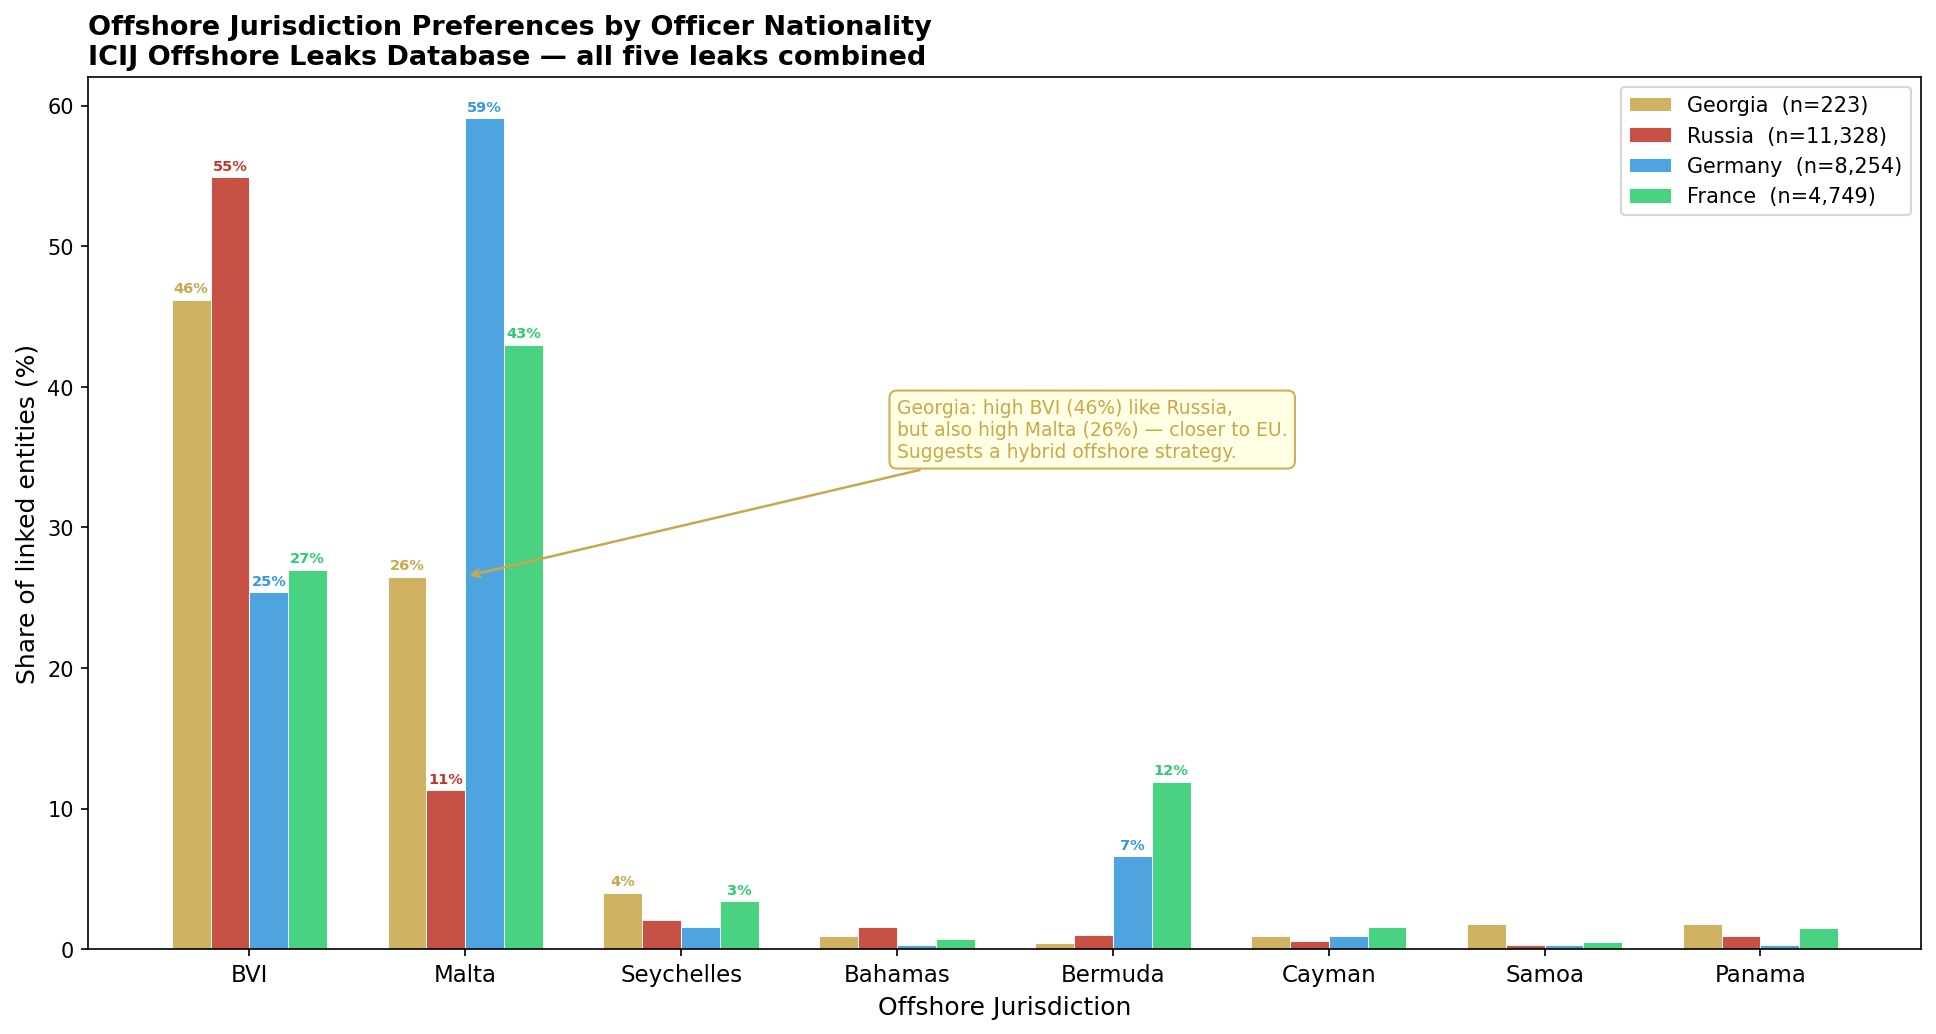
\includegraphics[width=\linewidth]{viz1_jurisdiction_profile.png}
\caption{Offshore jurisdiction preferences by officer nationality, all five leaks combined. Georgia's BVI share (46\%) approaches Russia's (55\%) while its Malta share (26\%) far exceeds Russia's (11\%) and approaches EU levels---a dual-track pattern unique to Georgia in this comparison set.}
\label{fig:jurisdictions}
\end{figure}

\textit{Temporal dynamics.} Figure~\ref{fig:timeline} shows annual new incorporations linked to Georgian officers, 1991--2018. Opaque-haven use accelerates from 2006 and peaks at 16 new entities in 2014, two years after the Georgian Dream party's October 2012 electoral victory and amid its consolidation of power. Malta-registered (semi-transparent) entities appear across the whole period, predating Ivanishvili's 2012 entry into politics, suggesting the EU-adjacent track reflects longstanding wealth-manager routing rather than post-political diversification. Incorporations decline after the 2016 Panama Papers release, consistent with a disclosure-driven chilling effect---a pattern to be tested, not assumed.

\begin{figure}[h!]
\centering

\includegraphics[width=\linewidth]{viz2_georgian_timeline.png}
\caption{Georgian-linked offshore entity incorporations by year, coloured by jurisdiction type. Opaque-haven use peaks at 16 entities in 2014; the Malta-heavy semi-transparent track predates the Ivanishvili era. Dashed lines mark Ivanishvili's 2004 return, the 2012 Georgian Dream victory, and the 2016 Panama Papers. $n=187$ entities with parseable incorporation dates (36 excluded for missing dates).}
\label{fig:timeline}
\end{figure}

\textit{Strategy similarity.} Table~\ref{tab:similarity} reports pairwise cosine similarities. Georgia--Russia (0.66) exceeds the Georgia--EU average (0.45). Georgia's closest analog is Belarus (0.93), then Latvia (0.81). The network (Fig.~\ref{fig:network}) shows two post-Soviet sub-patterns: a high-blacklist, low-EU-adjacent pairing (Russia--Belarus, 0.84) and an intermediate region where Georgia and Latvia sit. Latvia's high EU-adjacent share pulls it toward Germany (0.85), whereas Georgia's higher blacklist share and intermediary concentration keep it nearer the Russia--Belarus axis.

\begin{table}[h!]
\centering
\caption{Pairwise cosine similarity of offshore strategy vectors. Values $\geq 0.70$ in bold.}
\label{tab:similarity}
\begin{tabular}{lrrrrrr}
 & GEO & LVA & BLR & RUS & DEU & FRA \\
\midrule
GEO & 1.00 & \textbf{0.81} & \textbf{0.93} & 0.66 & 0.55 & 0.34 \\
LVA &      & 1.00 & 0.59 & 0.20 & \textbf{0.85} & 0.37 \\
BLR &      &      & 1.00 & \textbf{0.84} & 0.35 & 0.16 \\
RUS &      &      &      & 1.00 & 0.16 & 0.34 \\
DEU &      &      &      &      & 1.00 & 0.58 \\
FRA &      &      &      &      &      & 1.00 \\
\bottomrule
\end{tabular}
\end{table}

\begin{figure}[h!]
\centering
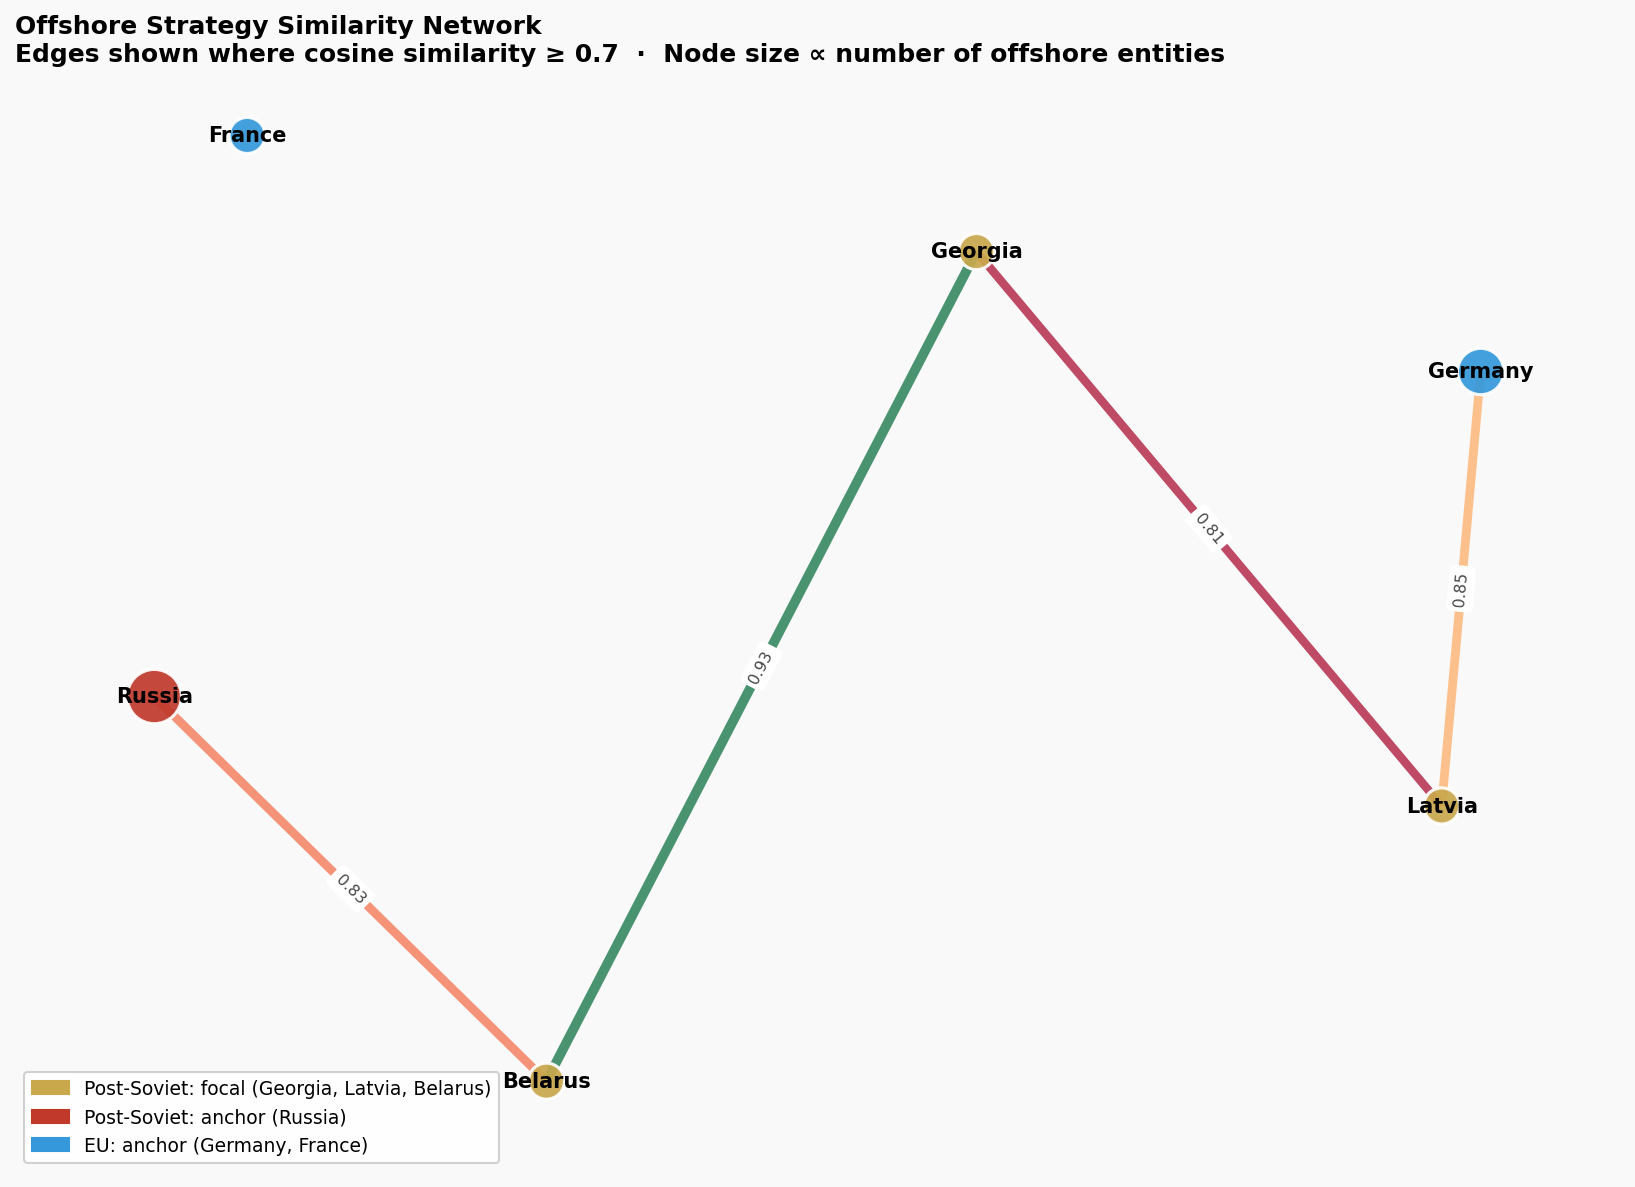
\includegraphics[width=\linewidth]{viz3_similarity_networks.png}
\caption{Offshore strategy similarity network. Edges shown where cosine similarity $\geq 0.70$; node size proportional to entity count. Georgia links strongly to Belarus (0.93) and Latvia (0.81) but not, at this threshold, to Russia or the EU anchors.}
\label{fig:network}
\end{figure}

\textit{Strategy fingerprints.} Figure~\ref{fig:radar} renders the normalized vectors as a radar plot. Russia's profile is dominated by blacklist share; France's is the inverse, with high entropy and a near-zero HHI. Georgia is distinctively wide on two axes at once---near-maximal intermediary HHI and elevated blacklist share---while still extending toward EU-adjacent share. Its raw HHI (0.068) is the highest in the set: about $2.9\times$ Russia's (0.024) and $8\times$ France's (0.008). Read alongside Chang et al.\ (2023), this concentration suggests Georgian structures are routed through a narrow set of wealth managers, the same intermediary bottleneck their network analysis identifies as characteristic of politically exposed, autocratic-regime clients \cite{chang2023}.

\begin{figure}[h!]
\centering
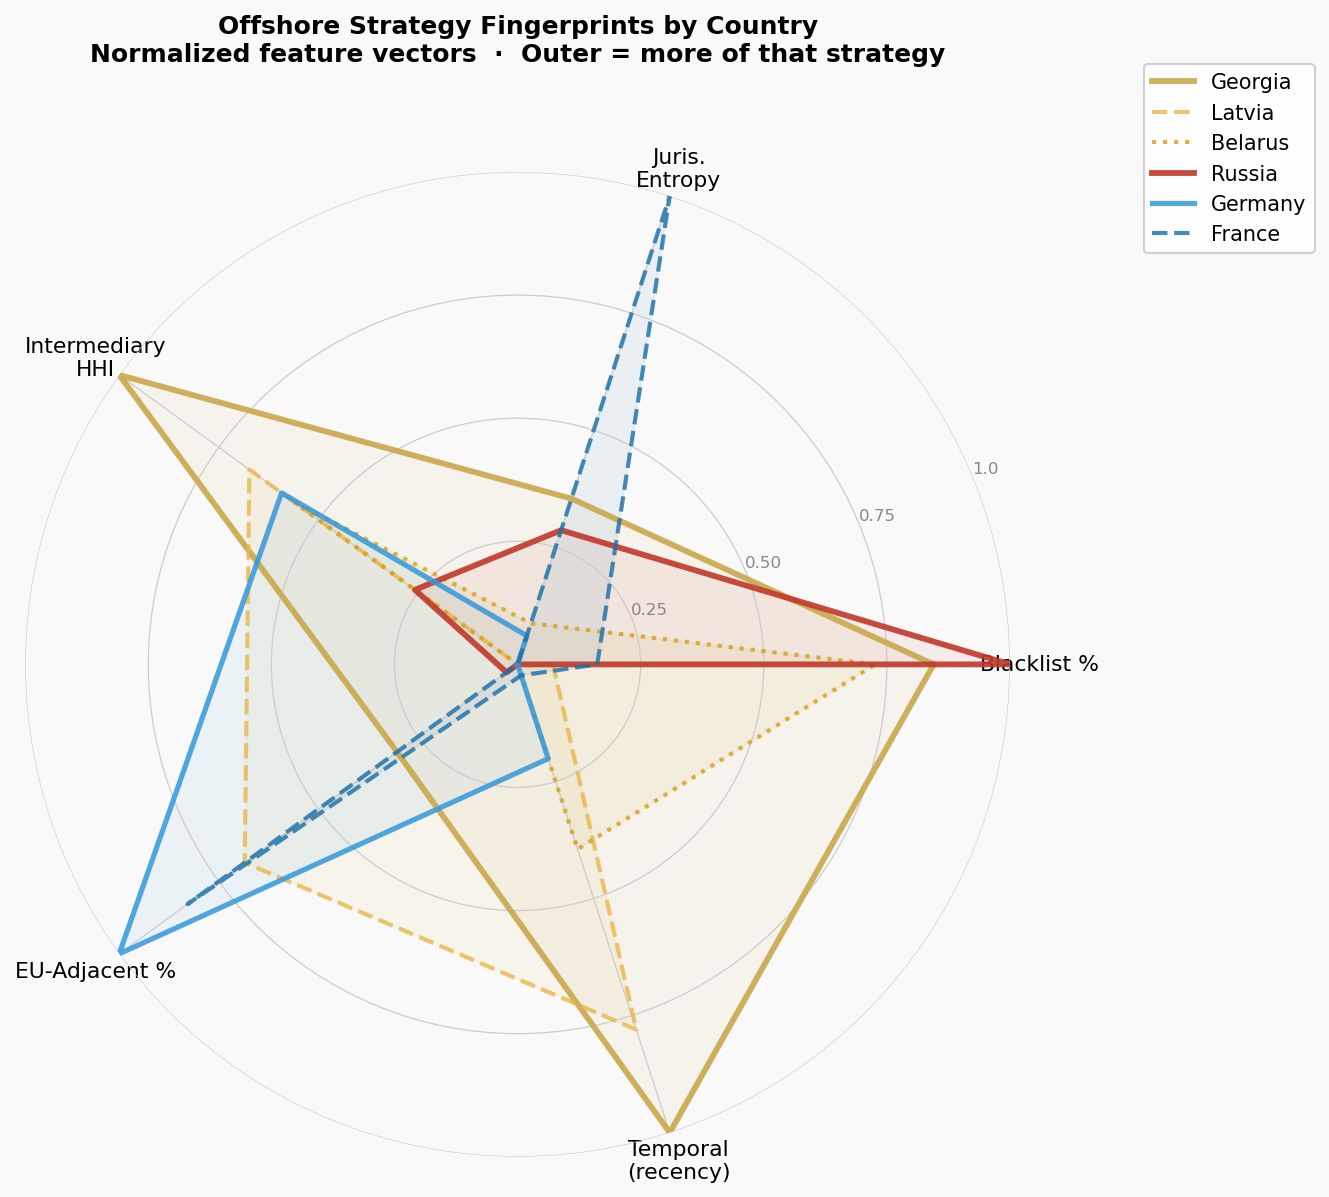
\includegraphics[width=\linewidth]{viz4_radar_chart.png}
\caption{Offshore strategy fingerprints by country. Normalized feature vectors; outer edge = more of that strategy. Georgia is uniquely wide on both blacklist share and intermediary HHI while also extending toward EU-adjacent share.}
\label{fig:radar}
\end{figure}

\section*{Discussion}

Three findings stand out. First, Georgian offshore actors pursue a genuinely dual-track strategy---combining opaque havens and EU-adjacent jurisdictions---that fits neither a pure Russian nor a pure EU template. Second, despite this hybridity, Georgia's strategy vector sits closer to Russia's than to the EU's, and opaque-haven use accelerates during the Georgian Dream consolidation, consistent with (though not proof of) post-Soviet inheritance reinforced by domestic political incentives. Third, Georgia's exceptionally high intermediary concentration echoes the wealth-manager bottleneck Chang et al.\ associate with autocratic-regime clients, suggesting the structural signature of post-Soviet capital persists even under formal EU orientation.

These conclusions are bounded. The Georgian sample is small ($n=223$ entities), so all results are descriptive; country-code attribution conflates recording practice with citizenship; and the design supports no causal identification---the correlation between incorporation peaks and political events is equally consistent with offshore infrastructure enabling political activity as with the reverse. Future work should (i) incorporate the Tax Justice Network Financial Secrecy Index to convert the categorical jurisdiction variable into a continuous secrecy score for regression, (ii) use the World Bank Worldwide Governance Indicators to contextualize the temporal series, as in the cross-national approach of Chang et al.\ (2025) \cite{chang2025}, and (iii) apply fuzzy name matching to build officer-level panels that test whether individual trajectories shift across political transitions.

\dataavail{All analysis code and output figures are available in the project repository. Raw data are available from the ICIJ at \url{offshoreleaks.icij.org/pages/database}.}

\acknow{Data are drawn from the ICIJ Offshore Leaks Database. The author thanks the QSS~20 teaching staff for guidance.}

\showacknow

\begin{thebibliography}{9}

\bibitem{alstadsaeter2019}
Alstad{\ae}ter A, Johannesen N, Zucman G (2019) Tax evasion and inequality. \textit{Am Econ Rev} 109(6):2073--2103.

\bibitem{chang2023}
Chang HCH, Harrington B, Fu F, Rockmore DN (2023) Complex systems of secrecy: the offshore networks of oligarchs. \textit{PNAS Nexus} 2(3):pgad051.

\bibitem{chang2025}
Chang HCH, Harrington B, Rockmore DN (2025) Secrecy strategies: global patterns in elites' quest for confidentiality in offshore finance. \textit{PLoS ONE} 20(7):e0326228.

\bibitem{zucman2015}
Zucman G (2015) \textit{The Hidden Wealth of Nations: The Scourge of Tax Havens} (Univ Chicago Press, Chicago).

\bibitem{novokmet2018}
Novokmet F, Piketty T, Zucman G (2018) From Soviets to oligarchs: inequality and property in Russia 1905--2016. \textit{J Econ Inequal} 16(2):189--223.

\end{thebibliography}

\clearpage
\section*{Appendix: Agentic Analysis}

\subsection*{Workflow overview}

I used two AI assistants during this project. Claude Chatbot helped with the research workflow: locating and summarizing relevant literature, developing the pandas analysis plan, designing exploratory data-analysis steps, and drafting code ideas for \path{code/01_analysis_and_visualizations.ipynb}. Codex was used later inside the GitHub repository to prepare the public-facing website, connect the output figures to the site, review repository organization, and compile the final LaTeX PDF from \path{latex/Research_mathematics.tex}. This appendix documents what I asked, what I accepted, what I changed, and where the assistants produced errors that required correction. Representative reconstructed excerpts from the workflow appear below.

\subsection*{What I asked the assistants to do}

The requests fell into five categories, roughly in the order the project developed.

\begin{enumerate}
  \item \textbf{Research and source orientation.} I asked Claude to help identify scholarly sources on offshore finance, oligarchic wealth, tax evasion, and post-Soviet capital. Claude helped me connect the project to Zucman (2015), Alstad{\ae}ter, Johannesen, and Zucman (2019), Novokmet, Piketty, and Zucman (2018), and Chang, Harrington, Fu, and Rockmore (2023).
  \item \textbf{Reproducible data loading.} I asked Claude for a notebook structure that would locate the raw ICIJ files across machines without hardcoding one absolute path, since the raw offshore leaks data are too large to track in GitHub. The resulting notebook logic checks multiple likely data locations and raises an informative \texttt{FileNotFoundError} when the files cannot be found.
  \item \textbf{Feature design and EDA.} I described the theoretical contrast between post-Soviet opacity and EU-adjacent tax efficiency. Claude suggested turning that idea into measurable features: blacklisted-jurisdiction share, Shannon entropy of jurisdiction diversity, intermediary Herfindahl--Hirschman index (HHI), EU-adjacent jurisdiction share, and temporal recency. These ideas became the core of \path{code/01_analysis_and_visualizations.ipynb}.
  \item \textbf{Figures and manuscript materials.} I asked Claude for help generating four publication-style visualizations from the notebook: \path{output/viz1_jurisdiction_profile.png}, \path{output/viz2_georgian_timeline.png}, \path{output/viz3_similarity_networks.png}, and \path{output/viz4_radar_chart.png}. I then used those figures in the LaTeX manuscript.
  \item \textbf{Website and final repository preparation.} I asked Codex to work directly in the repository to build the website files \path{app/page.jsx}, \path{app/layout.jsx}, and \path{app/globals.css}; copy figure assets into \path{public/assets/}; check that repository files were named clearly; and compile \path{latex/Research_mathematics.tex} into the final PDF.
\end{enumerate}

\subsection*{Representative assistant exchanges}

\begin{quote}
\textbf{Me:} ``Claude, I have ICIJ CSV files but the raw data will not be committed to GitHub. Can you help me make the notebook portable?''\\
\textbf{Claude:} ``Use a \texttt{candidate\_paths} list and test each location before loading. Keep the notebook repo-relative first, then check local Desktop/Downloads-style paths. If no path works, raise a \texttt{FileNotFoundError} that prints every searched path.''\\
\textbf{Accepted result:} I used this idea in \path{code/01_analysis_and_visualizations.ipynb} so the notebook explains where it expects the ICIJ data.
\end{quote}

\begin{quote}
\textbf{Me:} ``Claude, I want to compare Georgia with Russia and EU countries, but Russia has far more entities. What similarity measure should I use?''\\
\textbf{Claude:} ``Represent each country as a normalized strategy vector, then use cosine similarity. This compares the direction of the strategy profile rather than the raw country size.''\\
\textbf{Accepted result:} I kept the cosine-similarity matrix and used it to compare Georgia with Russia, Latvia, Belarus, Germany, and France.
\end{quote}

\begin{quote}
\textbf{Me:} ``Codex, create a website from the final project outputs and make sure it uses the actual visualizations.''\\
\textbf{Codex:} ``I will build the page in \path{app/page.jsx}, put global styling in \path{app/globals.css}, and reference copied images from \path{public/assets/} so the deployed site does not depend on notebook paths.''\\
\textbf{Accepted result:} I used the Codex-generated website structure and kept the figure assets aligned with the four manuscript visualizations.
\end{quote}

\subsection*{What I accepted}

I accepted Claude's feature-vector framework because it translated the substantive question into measurable quantities. The HHI feature was especially useful because intermediary concentration became one of the clearest ways to distinguish Georgia from both Russia and Western European reference countries. I also accepted the cosine-similarity approach because it reduced the effect of the large entity-count gap between Russia and Georgia. From Codex, I accepted the website structure in \path{app/page.jsx}, the use of \path{public/assets/} for visualization files, and the final repository checks that made the project easier to inspect.

\subsection*{What I rejected or modified}

\begin{enumerate}
  \item \textbf{Comparison-country scope.} Claude initially suggested expanding the comparison set beyond the post-Soviet/EU frame. I rejected that because the paper's design depends on a focused comparison among Georgia, Russia, Latvia, Belarus, Germany, and France.
  \item \textbf{Overgeneral literature claims.} Early AI-assisted summaries made the literature sound more directly about Georgia than it actually was. I revised the framing so the paper claims a narrower contribution: it positions Georgia in a measured offshore-strategy space rather than claiming that prior literature ignored the topic entirely.
  \item \textbf{Website wording.} Codex initially drafted some website language in a promotional style. I changed it so the site presented the research findings, figures, and repository materials more directly.
\end{enumerate}

\subsection*{Where the assistants went wrong}

\begin{enumerate}
  \item \textbf{Date parsing.} Claude initially treated incorporation dates as if one date format would cover the dataset. This produced missing values for records that used a different format. I corrected the notebook logic to parse dates more flexibly and then checked the number of usable Georgian incorporation years.
  \item \textbf{Citation accuracy.} Some AI-assisted draft language overstated what specific sources showed. I checked the claims against the original publications and rewrote the literature review so Alstad{\ae}ter, Johannesen, and Zucman (2019), Chang et al.\ (2023), and Chang, Harrington, and Rockmore (2025) were described accurately.
  \item \textbf{Unverified numbers.} When I asked for table improvements, the assistant suggested adding values that had not all been computed in the notebook. I removed unsupported cells and kept the manuscript tables tied to verified analysis output.
\end{enumerate}

\subsection*{Reflection}

The assistants were most useful for scaffolding code, proposing measurable features, organizing the website, and checking that the final repository was understandable to a reviewer. They were least reliable when summarizing literature or filling in quantitative details without direct verification. For that reason, I treated AI output as a draft rather than as evidence. Every empirical value in the paper was checked against \path{code/01_analysis_and_visualizations.ipynb} or the generated figures, and every source claim was reviewed against the cited publication before inclusion in the final manuscript.

\end{document}
